\chapter{Simulation Environment}

\section{Full-car Model}\label{env:full_car}

  \begin{figure}[ht]
    \centering
    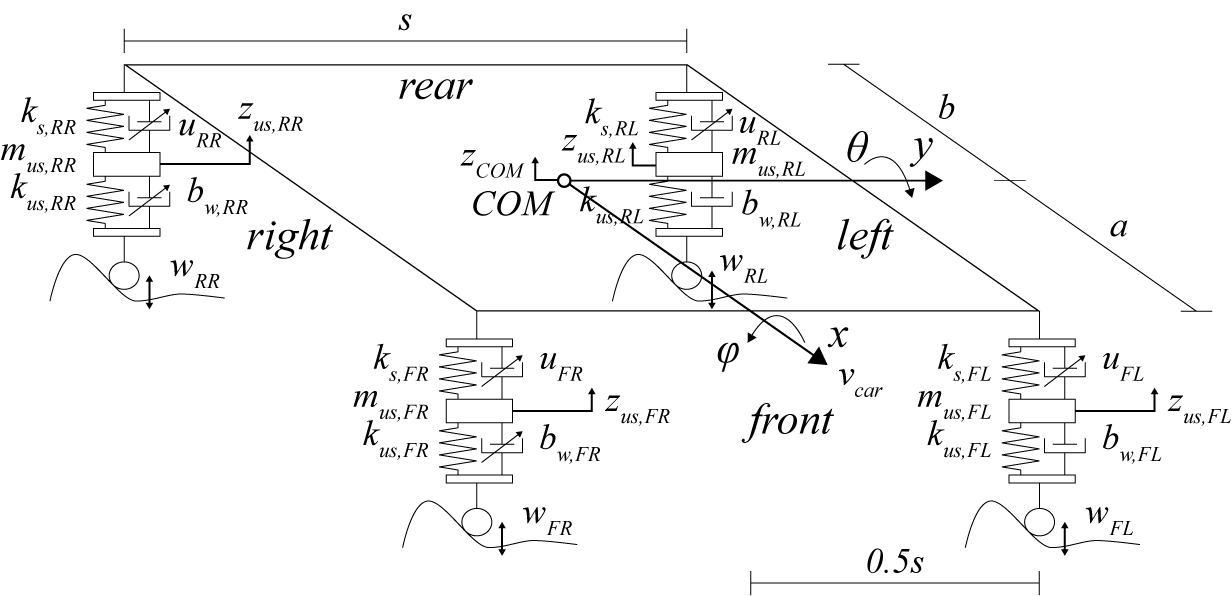
\includegraphics[width=0.8\textwidth]{figures/full_car.png}
    \caption{Full car dynamics diagram}
    \label{fig:full_car}
  \end{figure}

  The nonlinear full car model with semi-active suspensions in \cite{zhu2006chaotic} is adopted for the simulation. The target system can be described as follows. 
  \begin{eqnarray*} \label{eq:basic}
    \dot{x} = f(x,u)
  \end{eqnarray*}
  where 
  \begin{equation*}
    \begin{split}
      x = &[z_{com}, \dot{z}_{com}, \phi, \dot{\phi}, \theta, \dot{\theta},\\ &z_{us,FL},\dot{z}_{us,FL},z_{us,FR},\dot{z}_{us,FR},z_{us,RL},\dot{z}_{us,RL},z_{us,RR},\dot{z}_{us,RR}]^T\\
      = &[x_1,x_2,x_3,x_4,x_5,x_6,x_7,x_8,x_9,x_{10},x_{11},x_{12},x_{13},x_{14}]^T.
    \end{split}
  \end{equation*}
  
  Throughout this thesis, the system parameters of the vehicle model are in Table.~\ref{table:full_car_parameters}. The spring constants and damping constants are assumed to be identical for all suspensions.
  
  \begin{table}[ht!]
    \caption{Vehicle model parameters}
    \label{table:full_car_parameters}
    \scriptsize%
    {\raggedright COM* : Center of mass \par}
    \centering%
    \begin{tabu}{%
        c%
        *{7}{l}%
        *{2}{c}%
      }
      \toprule
      Parameter& Description  & Value \\
      \midrule
      $m_s$    & Mass of sprung body   & $1000\;kg$ \\
      \midrule
      $m_{us}$ & Mass of unsprung body (tires) & $50\;kg$ \\
      \midrule
      $I_{xx}$ & Mass moment of inertia in x axis             & $150 \;kg m^s$ \\
      \midrule
      $I_{yy}$ & Mass moment of inertia in y axis             & $346.875\; kg m^s$ \\
      \midrule
      $a$      & Length from the front of body to the COM* & $0.975 \; m$ \\
      \midrule
      $b$      & Length from the rear of body to the COM* & $0.975 \; m$ \\
      \midrule
      $s$      & Width of the body & $1.2 m$ \\
      \midrule
      $k_{sp}$ & Spring constant of shock absorbers & $2.1\;kgf/mm$ \\
      \midrule
      $c_{sp}$ & Nominal damping constant of shock absorbers & $10\;Ns/m$ \\
      \midrule
      $k_{t}$  & Spring constant of tires & $30\;kgf/mm$ \\
      \midrule
      $c_{t}$  & Damping constant of tires & $50\;Ns/m$ \\
      \bottomrule
    \end{tabu}
  
  \end{table}